\documentclass[12pt,letterpaper]{report}
\usepackage[margin=1in]{geometry}
\usepackage{titlesec}
\usepackage{amsmath}
\usepackage{amssymb}
\usepackage[colorlinks=true,urlcolor=black,linkcolor=black]{hyperref}
\usepackage{graphicx}
\usepackage{textcomp}
% extra packages you need
\usepackage{graphicx}
\usepackage{listings}
\usepackage{algorithm}
\usepackage{algorithmic}
\usepackage{amsmath}
\usepackage{latexsym}
\usepackage{amsfonts}
\usepackage[normalem]{ulem}
\usepackage{array}
\usepackage{amssymb}
\usepackage{subfig}
\usepackage{wrapfig}
\usepackage{wasysym}
\usepackage{enumitem}
\setlist[itemize]{after=\vspace{-0.50\baselineskip},before=\vspace{-0.95\baselineskip}}
\newlist{ucmenum}{enumerate}{1}
\setlist[ucmenum]{label=\arabic*,after=\vspace{-0.50\baselineskip},before=\vspace{-0.95\baselineskip}}
\usepackage{adjustbox}
\usepackage{ragged2e}
\usepackage{hhline}
\usepackage[svgnames,table]{xcolor}
\usepackage{tikz}
\usepackage{longtable}
\usepackage{changepage}
\usepackage{setspace}
\usepackage{multicol}
\usepackage{tabto}
\usepackage{float}
\usepackage{multirow}
\usepackage{makecell}
\usepackage{fancyhdr}
\usepackage[toc,page]{appendix}
\usepackage[utf8]{inputenc}
\usepackage{flowchart}
\usepackage{apacite}
\usepackage{color}
\makeglossaries

\titleformat{\chapter}{\bf\huge}{\thechapter}{20pt}{\huge\vspace{-.5em}}

\begin{document}
\title{Software Measurement (SOEN6611)\\[.5em]
Summer 2023\\[.5em]
Descriptive Statistics\\[.5em]
Team "Amsterdam Cartel"\\[.5em]
Deliverable 1}
\author{Unnati Chaturvedi, Mengqi Liu, Lei Zhou, Hema Reddy Mupppidi}
\maketitle

\pagenumbering{roman}
\setcounter{page}{0}

\tableofcontents

\chapter*{List of Symbols and Abbreviations}\addcontentsline{toc}{chapter}{List of Symbols and Abbreviations}



% delete these example entries
\noindent\begin{tabular}{ll}
% $\mathbb{R}$ & The set of real numbers (example)\\
% $\|\cdot\|_F$ & Frobenius norm (example)\\
GQM & Goal Question Metric\\
UC & Use Case

\end{tabular}

% delete this section if no figures
\listoffigures\addcontentsline{toc}{chapter}{List of Figures}
% This will automatically be populated if you included figures in your report.


%%%%%%%%%%%%%%%%%%%%%%%%%%%%%
\chapter{Background Information}
To develop the Sales Analytics System, named METRICSTICS, a critical system will be implemented in order to comprehensively analyze sales performance.This system will examine statistical analysis of sales data to empower the sales management team in effectively monitoring sales trends over time, conducting thorough analyses of sales history, and making informed decisions based on the insights gained. Both sales staff and sales administration personnel will have access to METRICSTICS, allowing the sales team to diligently input sales data and the sales manager to effortlessly access statistical information for specific time periods. Additionally, METRICSTICS will enable the generation of comprehensive reports on a monthly, quarterly, and yearly basis, which will be presented to the board of members.		 	 	 	

*Note: The key stakeholders for METRICSTICS are sales representatives, sales managers

%%%%%%%%%%%%%%%%%%%%%%%%%%%%%%
\chapter{Problem 1: Goal Question Metric}

\section{Goal}

Analyze the sale's history to understand the sale trend during the years to project METRICSTICS from the viewpoint of the sales manager.\\

\section{Smart}
Smart principle consists of : \\

\textbf{Specific}: The goal is specific because it clearly defines the objective of analyzing sales history and understanding sales trends. It focuses on providing insights from the sales manager's perspective, allowing for targeted analysis.\\

\textbf{Measurable}: The goal is measurable as it can be evaluated based on the metrics and questions established. The metrics, such as yearly sales growth rate, seasonal sales variation, and product/service growth rate (see below).\\

\textbf{Achievable}: The goal is achievable because analyzing sales history and understanding sales trends is feasible through the collection and analysis of relevant sales data. With the proper tools and system in place (METRICSTICS), the sales manager can obtain the necessary insights.\\

\textbf{Relevant}: The goal is relevant to the sales manager's role and responsibilities. Understanding sales trends and projecting METRICSTICS helps the sales manager make informed decisions, optimize sales strategies, and set realistic targets for the future.\\

\textbf{Time-bound}: The goal is time-bound as it focuses on analyzing sales history over the years. It allows for the examination of trends and patterns within specific time periods and facilitates projecting METRICSTICS based on historical data.\\

Overall, the goal follows the SMART principle by being specific, measurable, achievable, relevant, and time-bound. This ensures that the goal is well-defined, trackable, attainable, aligned with the sales manager's responsibilities, and has a clear time frame for analysis.



\section{Question and Metric}

% delete this text


\begin{enumerate}
\item
   \begin{enumerate}
	\item Question: What is the average of sales monthly and quarterly?
    \item Metric: 
    \begin{enumerate}
        \item Average(Mean) monthly sales
        \item Average(Mean) quarterly sales
    \end{enumerate}
    \item Mechanism:
    \begin{enumerate}
    \item Owner = Sales Managers
    \item Frequency Collected = following the monthly report generation
    \item Frequency Reported = Monthly and Quarterly
    \end{enumerate}
\end{enumerate}

\item
    \begin{enumerate}
    \item Question: What is the biggest sales growth and decline rate this year by monthly and quarterly?
    \item Metric: 
        \begin{enumerate}
            \item Maximum monthly sales decline rate
            \item Minimum monthly sales decline rate\\Maximum quarterly sales decline rate
            \item Maximum quarterly sales decline rate\\Minimum quarterly sales decline rate
        \end{enumerate}
    \item Mechanism:
	\begin{enumerate}
    \item Owner = Sales Managers
    \item Frequency Collected = following the monthly report generation
    \item Frequency Reported = Monthly and Quarterly
    \end{enumerate}
\end{enumerate}

\item
    \begin{enumerate}
    \item Question: How to determine that each month's and quarter’s  sales experience growth or decline?
    \item Metric: 
        \begin{enumerate}
            \item compute the baseline(MAD) in terms of monthly and quarterly sale
            \item compare it in monthly sale and quarterly sale
        \end{enumerate}
    \item Mechanism:
	\begin{enumerate}
    \item Owner = Sales Managers
    \item Frequency Collected = following the monthly report generation
    \item Frequency Reported = Monthly and Quarterly
    \end{enumerate}
\end{enumerate}

\item
    \begin{enumerate}
    \item Question: Which month and quarter experienced the most significant sales change over the yea?
    \item Metric: 
        \begin{enumerate}
            \item  standard deviation of monthly and quarterly sales
        \end{enumerate}
    \item Mechanism:
	\begin{enumerate}
    \item Owner = Sales Managers
    \item Frequency Collected = following the monthly report generation
    \item Frequency Reported = Monthly and Quarterly
    \end{enumerate}
\end{enumerate}

\item
    \begin{enumerate}
    \item Question: Which month and quarter experienced the most significant sales change over the year? (standard deviation)(mean)
    \item Metric: 
        \begin{enumerate}
            \item  standard deviation of monthly and quarterly sales
        \end{enumerate}
    \item Mechanism:
	\begin{enumerate}
    \item Owner = Sales Managers
    \item Frequency Collected = following the monthly report generation
    \item Frequency Reported = Monthly and Quarterly
    \end{enumerate}
\end{enumerate}

\item
    \begin{enumerate}
    \item Question: How to calculate the top 10 items that customers purchased at least twice on this platform monthly and quarterly, sorted by the number of purchases?
    \item Metric: 
        \begin{enumerate}
            \item  Count the number of times each item is purchased in a month monthly and quaterly
            \item find the items purchased more than once and sort them by their purchasing times monthly and quaterly
        \end{enumerate}
    \item Mechanism:
	\begin{enumerate}
    \item Owner = Sales Managers
    \item Frequency Collected = following the monthly and quaterly report generation
    \item Frequency Reported = Monthly and Quarterly
    \end{enumerate}
\end{enumerate}

\item
    \begin{enumerate}
    \item Question: What is the most popular item monthly?
    \item Metric: 
        \begin{enumerate}
            \item  Count the number of times each item is purchased in a month and find the item with the highest count.
        \end{enumerate}
    \item Mechanism:
	\begin{enumerate}
    \item Owner = Sales Managers
    \item Frequency Collected = following the monthly report generation
    \item Frequency Reported = Monthly
    \end{enumerate}
\end{enumerate}

\item
    \begin{enumerate}
    \item Question: In which city residents make the biggest purchases on this platform for the whole year?
    \item Metric: 
        \begin{enumerate}
            \item  Count the number of purchases based on the city extracted from purchase addresses and find the city with the highest count.
        \end{enumerate}
    \item Mechanism:
	\begin{enumerate}
    \item Owner = Sales Managers
    \item Frequency Collected = following the yearly report generation
    \item Frequency Reported = Yearly
    \end{enumerate}
\end{enumerate}

\item
    \begin{enumerate}
    \item Question: How to determine the day of the year when people engage in the highest amount of shopping?
    \item Metric: 
        \begin{enumerate}
            \item  Count the number of purchases each day in a year and find the day with the highest count.
        \end{enumerate}
    \item Mechanism:
	\begin{enumerate}
    \item Owner = Sales Managers
    \item Frequency Collected = following the yearly report generation
    \item Frequency Reported = Yearly
    \end{enumerate}
\end{enumerate}

%%%%%%%%%%%%%%%%%%%%%%%%%%%%%%
\chapter{Problem 2: Use Case Model}
\section{Use Case Diagram}

\begin{figure}[h]
    \begin{center}
    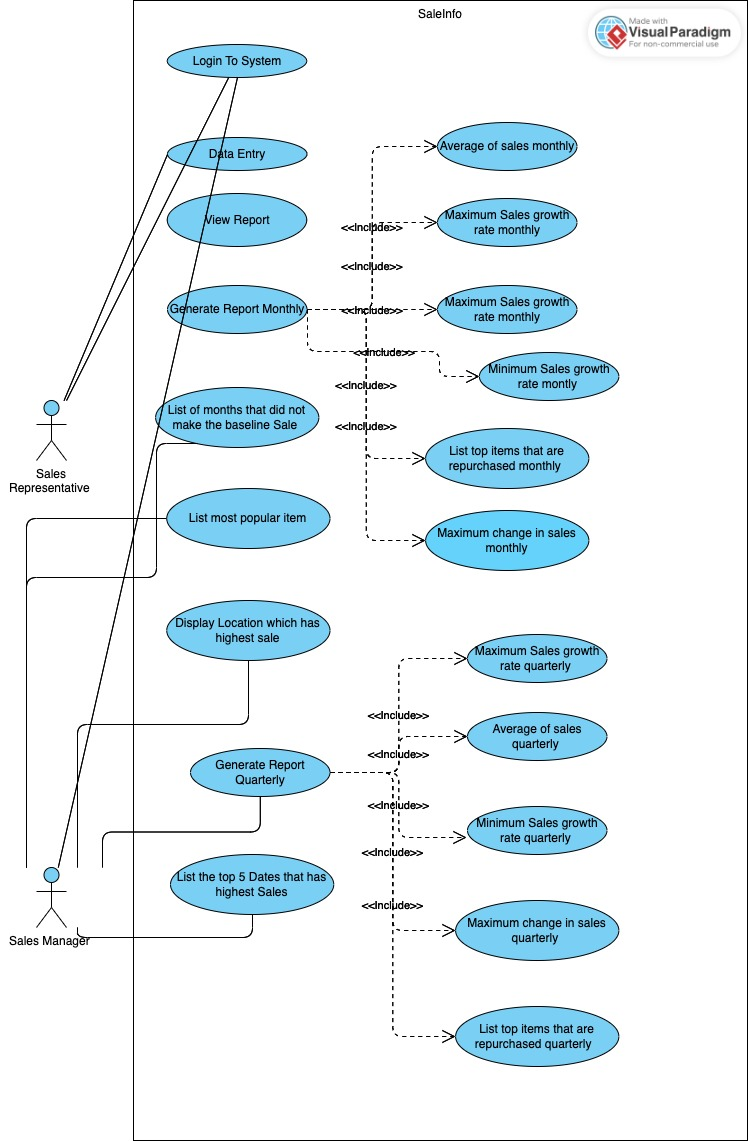
\includegraphics[width=0.5\linewidth]{14.jpg}
    \end{center}
       \caption{Use Case Model \label{Use Case Model}}
\end{figure}

\section{Use Cases}

\begin{table}[H]
 			\centering
\begin{tabular}{p{1.23in}p{4.87in}}
\hline
%row no:1
\multicolumn{1}{|p{1.23in}}{Use Case ID} & 
\multicolumn{1}{|p{4.87in}|}{UC-1} \\
\hhline{--}
%row no:2
\multicolumn{1}{|p{1.23in}}{Use Case Name} & 
\multicolumn{1}{|p{4.87in}|}{Log in to the System} \\
\hhline{--}
%row no:3
\multicolumn{1}{|p{1.23in}}{Primary Actors} & 
\multicolumn{1}{|p{4.87in}|}{\begin{itemize}
	\item Sales Representative \par 	\item Sales Manager
\end{itemize}} \\
\hhline{--}
%row no:4
\multicolumn{1}{|p{1.23in}}{Priority} & 
\multicolumn{1}{|p{4.87in}|}{High} \\
\hhline{--}
%row no:5
\multicolumn{1}{|p{1.23in}}{Description} & 
\multicolumn{1}{|p{4.87in}|}{User can login into the System.} \\
\hhline{--}
%row no:6
\multicolumn{1}{|p{1.23in}}{Pre-conditions} & 
\multicolumn{1}{|p{4.87in}|}{\begin{itemize}
	\item User has a valid account on the system.
\end{itemize}} \\
\hhline{--}
%row no:7
\multicolumn{1}{|p{1.23in}}{Post-conditions} & 
\multicolumn{1}{|p{4.87in}|}{\begin{itemize}
	\item User logged in successfully.
\end{itemize}} \\
\hhline{--}
%row no:8
\multicolumn{1}{|p{1.23in}}{Normal Flow} & 
\multicolumn{1}{|p{4.87in}|}{\begin{ucmenum}
	\item User open the login page of the system \par 	\item System displays the login page. \par 	\item User enters their username and their password. \par \item User clicks on $``$Login$"$ button. \par 	\item System checks the User’s credentials. \par 	\item System displays the homepage. \par 	\item User sees the homepage.
\end{ucmenum}} \\
\hhline{--}
\end{tabular}
 \end{table}


 \begin{table}[H]
 			\centering
\begin{tabular}{p{1.23in}p{4.87in}}
\hline
%row no:1
\multicolumn{1}{|p{1.23in}}{Use Case ID} & 
\multicolumn{1}{|p{4.87in}|}{UC-2} \\
\hhline{--}
%row no:2
\multicolumn{1}{|p{1.23in}}{Use Case Name} & 
\multicolumn{1}{|p{4.87in}|}{Data Entry} \\
\hhline{--}
%row no:3
\multicolumn{1}{|p{1.23in}}{Primary Actors} & 
\multicolumn{1}{|p{4.87in}|}{\begin{itemize}
	\item Sales Representative
\end{itemize}} \\
\hhline{--}
%row no:4
\multicolumn{1}{|p{1.23in}}{Priority} & 
\multicolumn{1}{|p{4.87in}|}{High} \\
\hhline{--}
%row no:5
\multicolumn{1}{|p{1.23in}}{Description} & 
\multicolumn{1}{|p{4.87in}|}{Sale Representatives are able to entry the data regarding the customer purchasing item.} \\
\hhline{--}
%row no:6
\multicolumn{1}{|p{1.23in}}{Pre-conditions} & 
\multicolumn{1}{|p{4.87in}|}{\begin{itemize}
	\item Sale Representative login to the system.
\end{itemize}} \\
\hhline{--}
%row no:7
\multicolumn{1}{|p{1.23in}}{Post-conditions} & 
\multicolumn{1}{|p{4.87in}|}{\begin{itemize}
	\item User successfully added data.
\end{itemize}} \\
\hhline{--}
%row no:8
\multicolumn{1}{|p{1.23in}}{Normal Flow} & 
\multicolumn{1}{|p{4.87in}|}{\begin{ucmenum}
	\item Users are able to enter the name of the item, purchase date, customer’s address, quantity of item, and etc. \par \item User click the submit button. \par 	\item System store the sale data to database. \par 	\item System redirect to data entry page again with empty input.
\end{ucmenum}} \\
\hhline{--}
\end{tabular}
 \end{table}

  \begin{table}[H]
 			\centering
\begin{tabular}{p{1.23in}p{4.87in}}
\hline
%row no:1
\multicolumn{1}{|p{1.23in}}{Use Case ID} & 
\multicolumn{1}{|p{4.87in}|}{UC-3} \\
\hhline{--}
%row no:2
\multicolumn{1}{|p{1.23in}}{Use Case Name} & 
\multicolumn{1}{|p{4.87in}|}{View The Statistics Result} \\
\hhline{--}
%row no:3
\multicolumn{1}{|p{1.23in}}{Primary Actors} & 
\multicolumn{1}{|p{4.87in}|}{\begin{itemize}
	\item Sale Manager
\end{itemize}} \\
\hhline{--}
%row no:4
\multicolumn{1}{|p{1.23in}}{Priority} & 
\multicolumn{1}{|p{4.87in}|}{High} \\
\hhline{--}
%row no:5
\multicolumn{1}{|p{1.23in}}{Description} & 
\multicolumn{1}{|p{4.87in}|}{Sales Manager is able to view the statistics result generated from the sales history data.} \\
\hhline{--}
%row no:6
\multicolumn{1}{|p{1.23in}}{Pre-conditions} & 
\multicolumn{1}{|p{4.87in}|}{\begin{itemize}
	\item Sales Manager is able to login to the system. Corresponding sales data are ready in the system.
\end{itemize}} \\
\hhline{--}
%row no:7
\multicolumn{1}{|p{1.23in}}{Post-conditions} & 
\multicolumn{1}{|p{4.87in}|}{\begin{itemize}
	\item User is able to see the report page.
\end{itemize}} \\
\hhline{--}
%row no:8
\multicolumn{1}{|p{1.23in}}{Normal Flow} & 
\multicolumn{1}{|p{4.87in}|}{\begin{ucmenum}
	\item User is able to see the report page. \par \item Users are able to enter the conditions for the report, like time duration or specific month, etc. \par 	\item User clicks the submit button to calculate the statistics. \par 	\item User is able to view the statistics results.
\end{ucmenum}} \\
\hhline{--}
\end{tabular}
 \end{table}

 
\begin{table}[H]
 			\centering
\begin{tabular}{p{1.23in}p{4.87in}}
\hline
%row no:1
\multicolumn{1}{|p{1.23in}}{Use Case ID} & 
\multicolumn{1}{|p{4.87in}|}{UC-4} \\
\hhline{--}
%row no:2
\multicolumn{1}{|p{1.23in}}{Use Case Name} & 
\multicolumn{1}{|p{4.87in}|}{Generate report in monthly } \\
\hhline{--}
%row no:3
\multicolumn{1}{|p{1.23in}}{Primary Actors} & 
\multicolumn{1}{|p{4.87in}|}{\begin{itemize}
	\item System itself or Sales Manager

\end{itemize}} \\
\hhline{--}
%row no:4
\multicolumn{1}{|p{1.23in}}{Priority} & 
\multicolumn{1}{|p{4.87in}|}{High} \\
\hhline{--}
%row no:5
\multicolumn{1}{|p{1.23in}}{Description} & 
\multicolumn{1}{|p{4.87in}|}{Sales Manager is able to generate the statistics report in both monthly and quarterly.} \\
\hhline{--}
%row no:6
\multicolumn{1}{|p{1.23in}}{Pre-conditions} & 
\multicolumn{1}{|p{4.87in}|}{\begin{itemize}
	\item Sales Manager is able to login to the system. Sales data is ready in the system.
\end{itemize}} \\
\hhline{--}
%row no:7
\multicolumn{1}{|p{1.23in}}{Post-conditions} & 
\multicolumn{1}{|p{4.87in}|}{\begin{itemize}
	\item User is able to generate the report.
\end{itemize}} \\
\hhline{--}
%row no:8
\multicolumn{1}{|p{1.23in}}{Normal Flow} & 
\multicolumn{1}{|p{4.87in}|}{\begin{ucmenum}
	\item User is able to see the report page. \par \item Users are able to enter the conditions for the report, like time duration or specific month, etc. \par 	\item Or the sales manager sets the needed report and the system itself will generate on time.
\end{ucmenum}} \\
\hhline{--}
\end{tabular}
 \end{table}

 
\begin{table}[H]
 			\centering
\begin{tabular}{p{1.23in}p{4.87in}}
\hline
%row no:1
\multicolumn{1}{|p{1.23in}}{Use Case ID} & 
\multicolumn{1}{|p{4.87in}|}{UC-5} \\
\hhline{--}
%row no:2
\multicolumn{1}{|p{1.23in}}{Use Case Name} & 
\multicolumn{1}{|p{4.87in}|}{Generate report in quarterly } \\
\hhline{--}
%row no:3
\multicolumn{1}{|p{1.23in}}{Primary Actors} & 
\multicolumn{1}{|p{4.87in}|}{\begin{itemize}
	\item System itself or Sales Manager

\end{itemize}} \\
\hhline{--}
%row no:4
\multicolumn{1}{|p{1.23in}}{Priority} & 
\multicolumn{1}{|p{4.87in}|}{High} \\
\hhline{--}
%row no:5
\multicolumn{1}{|p{1.23in}}{Description} & 
\multicolumn{1}{|p{4.87in}|}{Sales Manager is able to generate the statistics report in both monthly and quarterly.} \\
\hhline{--}
%row no:6
\multicolumn{1}{|p{1.23in}}{Pre-conditions} & 
\multicolumn{1}{|p{4.87in}|}{\begin{itemize}
	\item Sales Manager is able to login to the system. Sales data is ready in the system.
\end{itemize}} \\
\hhline{--}
%row no:7
\multicolumn{1}{|p{1.23in}}{Post-conditions} & 
\multicolumn{1}{|p{4.87in}|}{\begin{itemize}
	\item User is able to generate the report.
\end{itemize}} \\
\hhline{--}
%row no:8
\multicolumn{1}{|p{1.23in}}{Normal Flow} & 
\multicolumn{1}{|p{4.87in}|}{\begin{ucmenum}
	\item User is able to see the report page. \par \item Users are able to enter the conditions for the report, like time duration or specific month, etc. \par 	\item Or the sales manager sets the needed report and the system itself will generate on time.
\end{ucmenum}} \\
\hhline{--}
\end{tabular}
 \end{table}


\begin{table}[H]
 			\centering
\begin{tabular}{p{1.23in}p{4.87in}}
\hline
%row no:1
\multicolumn{1}{|p{1.23in}}{Use Case ID} & 
\multicolumn{1}{|p{4.87in}|}{UC-6} \\
\hhline{--}
%row no:2
\multicolumn{1}{|p{1.23in}}{Use Case Name} & 
\multicolumn{1}{|p{4.87in}|}{List of months that did not make the baseline Sale requirement} \\
\hhline{--}
%row no:3
\multicolumn{1}{|p{1.23in}}{Primary Actors} & 
\multicolumn{1}{|p{4.87in}|}{\begin{itemize}
	\item Sale Manager

\end{itemize}} \\
\hhline{--}
%row no:4
\multicolumn{1}{|p{1.23in}}{Priority} & 
\multicolumn{1}{|p{4.87in}|}{Low} \\
\hhline{--}
%row no:5
\multicolumn{1}{|p{1.23in}}{Description} & 
\multicolumn{1}{|p{4.87in}|}{Users is able to see list of  months whose sales requirement were not met.} \\
\hhline{--}
%row no:6
\multicolumn{1}{|p{1.23in}}{Pre-conditions} & 
\multicolumn{1}{|p{4.87in}|}{\begin{itemize}
	\item Users have a valid account on the system.Sales data is ready in the system.
\end{itemize}} \\
\hhline{--}
%row no:7
\multicolumn{1}{|p{1.23in}}{Post-conditions} & 
\multicolumn{1}{|p{4.87in}|}{\begin{itemize}
	\item User is able to generate the list successfully.
\end{itemize}} \\
\hhline{--}
%row no:8
\multicolumn{1}{|p{1.23in}}{Normal Flow} & 
\multicolumn{1}{|p{4.87in}|}{\begin{ucmenum}
	\item Users are able to see the report page. \par \item Users are able to see the sales of a selected month from the list.
\end{ucmenum}} \\
\hhline{--}
\end{tabular}
 \end{table}


\begin{table}[H]
 			\centering
\begin{tabular}{p{1.23in}p{4.87in}}
\hline
%row no:1
\multicolumn{1}{|p{1.23in}}{Use Case ID} & 
\multicolumn{1}{|p{4.87in}|}{UC-7} \\
\hhline{--}
%row no:2
\multicolumn{1}{|p{1.23in}}{Use Case Name} & 
\multicolumn{1}{|p{4.87in}|}{List most popular Item} \\
\hhline{--}
%row no:3
\multicolumn{1}{|p{1.23in}}{Primary Actors} & 
\multicolumn{1}{|p{4.87in}|}{\begin{itemize}
	\item Sale Manager

\end{itemize}} \\
\hhline{--}
%row no:4
\multicolumn{1}{|p{1.23in}}{Priority} & 
\multicolumn{1}{|p{4.87in}|}{Low} \\
\hhline{--}
%row no:5
\multicolumn{1}{|p{1.23in}}{Description} & 
\multicolumn{1}{|p{4.87in}|}{Users is able to see the most popular item.} \\
\hhline{--}
%row no:6
\multicolumn{1}{|p{1.23in}}{Pre-conditions} & 
\multicolumn{1}{|p{4.87in}|}{\begin{itemize}
	\item Users have a valid account on the system.Sales data is ready in the system.
\end{itemize}} \\
\hhline{--}
%row no:7
\multicolumn{1}{|p{1.23in}}{Post-conditions} & 
\multicolumn{1}{|p{4.87in}|}{\begin{itemize}
	\item User is able to generate the most popular item.
\end{itemize}} \\
\hhline{--}
%row no:8
\multicolumn{1}{|p{1.23in}}{Normal Flow} & 
\multicolumn{1}{|p{4.87in}|}{\begin{ucmenum}
	\item Users are able to see the report page. \par \item Users are able to see the sales of a selected item.
\end{ucmenum}} \\
\hhline{--}
\end{tabular}
 \end{table}

 
\begin{table}[H]
 			\centering
\begin{tabular}{p{1.23in}p{4.87in}}
\hline
%row no:1
\multicolumn{1}{|p{1.23in}}{Use Case ID} & 
\multicolumn{1}{|p{4.87in}|}{UC-8} \\
\hhline{--}
%row no:2
\multicolumn{1}{|p{1.23in}}{Use Case Name} & 
\multicolumn{1}{|p{4.87in}|}{Display Location which has highest sale} \\
\hhline{--}
%row no:3
\multicolumn{1}{|p{1.23in}}{Primary Actors} & 
\multicolumn{1}{|p{4.87in}|}{\begin{itemize}
	\item Sale Manager

\end{itemize}} \\
\hhline{--}
%row no:4
\multicolumn{1}{|p{1.23in}}{Priority} & 
\multicolumn{1}{|p{4.87in}|}{Low} \\
\hhline{--}
%row no:5
\multicolumn{1}{|p{1.23in}}{Description} & 
\multicolumn{1}{|p{4.87in}|}{Users is able to see the Location which has highest sale.} \\
\hhline{--}
%row no:6
\multicolumn{1}{|p{1.23in}}{Pre-conditions} & 
\multicolumn{1}{|p{4.87in}|}{\begin{itemize}
	\item Users have a valid account on the system.Sales data is ready in the system.
\end{itemize}} \\
\hhline{--}
%row no:7
\multicolumn{1}{|p{1.23in}}{Post-conditions} & 
\multicolumn{1}{|p{4.87in}|}{\begin{itemize}
	\item User is able to generate the most popular Location.
\end{itemize}} \\
\hhline{--}
%row no:8
\multicolumn{1}{|p{1.23in}}{Normal Flow} & 
\multicolumn{1}{|p{4.87in}|}{\begin{ucmenum}
	\item Users are able to see the report page. \par \item Users are able to see the sales of a selected Location.
\end{ucmenum}} \\
\hhline{--}
\end{tabular}
 \end{table}


\begin{table}[H]
 			\centering
\begin{tabular}{p{1.23in}p{4.87in}}
\hline
%row no:1
\multicolumn{1}{|p{1.23in}}{Use Case ID} & 
\multicolumn{1}{|p{4.87in}|}{UC-9} \\
\hhline{--}
%row no:2
\multicolumn{1}{|p{1.23in}}{Use Case Name} & 
\multicolumn{1}{|p{4.87in}|}{List the top 5 Dates that has highest Sales} \\
\hhline{--}
%row no:3
\multicolumn{1}{|p{1.23in}}{Primary Actors} & 
\multicolumn{1}{|p{4.87in}|}{\begin{itemize}
	\item Sale Manager

\end{itemize}} \\
\hhline{--}
%row no:4
\multicolumn{1}{|p{1.23in}}{Priority} & 
\multicolumn{1}{|p{4.87in}|}{Low} \\
\hhline{--}
%row no:5
\multicolumn{1}{|p{1.23in}}{Description} & 
\multicolumn{1}{|p{4.87in}|}{Users is able to see the top 5 Dates that has highest Sales.} \\
\hhline{--}
%row no:6
\multicolumn{1}{|p{1.23in}}{Pre-conditions} & 
\multicolumn{1}{|p{4.87in}|}{\begin{itemize}
	\item Users have a valid account on the system.Sales data is ready in the system.
\end{itemize}} \\
\hhline{--}
%row no:7
\multicolumn{1}{|p{1.23in}}{Post-conditions} & 
\multicolumn{1}{|p{4.87in}|}{\begin{itemize}
	\item User is able to generate the most popular sale.
\end{itemize}} \\
\hhline{--}
%row no:8
\multicolumn{1}{|p{1.23in}}{Normal Flow} & 
\multicolumn{1}{|p{4.87in}|}{\begin{ucmenum}
	\item Users are able to see the report page. \par \item Users are able to see the sales of the top 5 dates displayed .
\end{ucmenum}} \\
\hhline{--}
\end{tabular}
 \end{table}



%%%%%%%%%%%%%%%%%%%%%%%%%%%%%%

\begin{thebibliography}{7}
    \addcontentsline{toc}{chapter}{Bibliography}

    % delete all of these example references, and replace them with references for your report.
    
    \bibitem{Lecture Slides} 
    Lecture Slides 
    \textit{Lecture slides"SOEN6611 Course Website”}.     
    
     \bibitem{Software Measurement Metrics} 
    Metrics.,
    \\\texttt{https://www.geeksforgeeks.org/software-measurement-and-metrics/}
    
    \bibitem{Use Case Diagram} 
    Use Case Diagram.,
    \\\texttt{https://www.visual-paradigm.com/guide/uml-unified-modeling-language/what is use case diagram/}

 
    

    
\end{thebibliography}

 
\textbf{{Github Repository}}

https://github.com/hemareddy123/SOEN\_6611\_Summer2023/tree/main

\end{document}
